
\documentclass[12pt]{article}
\usepackage{amsmath,amssymb,color,graphicx}
\usepackage{verbatim}
\textwidth=6.68in
\textheight=8.7in
\oddsidemargin 0.0in
\parindent=0in

\newtheorem{theorem}{Theorem} % added a "Theorem" environment  - A.Rad. Sept 26
\newtheorem{definition}{Definition}% added a "definition" environment - A.Rad. Sept 26
\newtheorem{example}[theorem]{Example}

\begin{document}
\pagestyle{empty}
\parskip=10pt
\def\xb{\bar{x}}
\begin{center}
{\Large \bf Lab 3: Iterated Function Systems}\\
{\it Math 112 -  Prof. Radunskaya} \\ 
\end{center}
{\bf Go through the lab with a partner.  (Each person should have their own computer if possible).  TURN IN THE ANSWERS TO NUMBER 6 - include your partner's name.
Do number 7 if you have time.}
\vskip 8pt
{\it Iterated Function Systems} are dynamical systems that are often used to generate fractals: sets with non-integer dimension.  In this Lab we will explore some of these systems in the plane.  Thus, our dynamical system will act on two-dimensional vectors, which we will denote by
$$ p = \left[\begin{array}{c}x \\y \end{array}\right] $$
\begin{enumerate}
\item Let $ p_0 = \left[\begin{array}{c}x_0 \\y_0 \end{array}\right] $ be a fixed point in the plane, and define the function
$$ A\left[\begin{array}{c}x \\y \end{array}\right] = \beta \left[\begin{array}{c}x - x_0 \\y - y_0 \end{array}\right] +  \left[\begin{array}{c}x_0 \\y_0 \end{array}\right] $$
or, in vector notation:  
$$ A(p) = \beta (p - p_0) + p_0$$
Show that, if $0 < \beta < 1$ then $p_0$ is the unique attracting fixed point of $A$.\\
{\it Hint: } First show that $A$ {\it contracts} distances, i.e. that $||A(p) - A(p_0)|| = \beta ||p - p_0 || $ where $|| \cdot ||$ denotes the {\it norm}
or length of the vector in ${\mathbb R}^2$: $|| \left[\begin{array}{c}x  \\y \end{array}\right] || = \sqrt{x^2 + y^2} $.
\vskip 4pt
\noindent
\begin{definition} Let $0 < \beta < 1$, and let $\{ p_1, \dots , p_n\}$ be a set of points in the plane. Let $A_i(p) = \beta(p - p_i) + p_i$ for $i = 1 \dots n$.
The set ${\cal A} = \{A_1 \dots A_n \}$ is an {\bf iterated function system}.
\end{definition}
An iterated function system (IFS)  is a dynamical system of a special sort.  The orbit of a point $p_0$ under the IFS is the sequence 
$p_0, p_1 = A_{X_1}(p_0), p_2 = A_{X_2}(p_1) , \dots $, where each $A_{X_i}$ is a {\it random} choice from ${\cal A}$.  (Note that by ``random" choice, we
mean that each $A_i$ has equal probability of begin chosen.
\begin{definition} The set of points in the plane to which an arbitrary orbit of an IFS converges is the {\bf attractor} for the system.
\end{definition}
{\it Note:}  Since the $A_i$'s are chosen randomly, we can only say that orbits converge {\it with a certain probability}.  Therefore we should say that an arbitrary orbit converges {\it with probability 1} to the attractor.
\item {\bf The Cantor  Set as an Attractor}
\\ We will use Matlab to generate the Cantor Middle Thirds set as the attractor of an IFS.
\begin{enumerate}
\item Open Matlab and select your 112 folder as the Current Directory.
\item {\bf Matlab basics:}\\
The command ``rand" generates a random number uniformly distributed between 0 and 1.  Try it, type:
\begin{verbatim}
>> rand
\end{verbatim}
{\it Note: Don't type the command prompt ``$>>$", and follow each line with ``enter" or ``return".}
\item If we want to generate a random integer between 1 and 47, say, we can multiply the rand number
by 47 and ``round up" using the ``ceiling" function:
\begin{verbatim}
>> ceil(47*rand)
\end{verbatim}
To generate a vector, v,  containing 7 of these numbers:
\begin{verbatim}
>> v=ceil(47*rand(1,7))
\end{verbatim}
Try this:
\begin{verbatim}
>> w = rand(3,4)
\end{verbatim}
To generate a vector, say $p = \left[\begin{array}{c}1 \\2\end{array}\right]$, type:
\begin{verbatim}
>> p = [1;2]
\end{verbatim}
{\bf TO DO:}  Try the same command with a comma instead of the semi-colon.  Explain to your partner what difference this makes.  Now try the same command with a semi-colon at the {\it end}.  Explain to your partner what difference this makes.\\
Vectors can be added or subtracted, as long as they are the same size.  They can also be multiplied by a scalar.  Type the following to see what it does:
\begin{verbatim}
>> q = [3;4];
>> p+q
>> p-q
>> 47*(p-.5*q)
\end{verbatim}
{\bf TO DO:} Explain to your partner why the following will give you an error:
\begin{verbatim}
>> w = [-1, 7];
>> p + w
\end{verbatim}
To switch from a column to a row vector, you can take the transpose:
\begin{verbatim}
>> ptrans = p'
\end{verbatim}
We'll also want to store a bunch of vectors in a matrix, and access them one by one.  To create a matrix, say, $P$, with
two rows and three columns:
\begin{verbatim}
P = [1 2 3; 4 5 6]
\end{verbatim}
Notice that the semicolon (``;") means ``start a new row".\\
To access the $(i,j)$th entry of $P$, type $P(i,j)$.  So, to get the entry in the first row, third column, you type:
\begin{verbatim}
P(1,3)
\end{verbatim}
To get the first column, use the shortcut ``:" to mean "all", so ``all rows, first column" gives the vector in the first column of $P$:
\begin{verbatim}
P(:,1)
\end{verbatim}
\item We will now create a file with the collection of $A_i$'s.  In the ``File" menu, select ``New M-file".  This will open the Editor Window.  Type the following:
\begin{verbatim}
function nextp = CantorIFS(p)

i=ceil(2*rand);
pset = [0 0; 1 0];
nextp = 1/3*p+2/3*pset(:,i);
\end{verbatim}
Save this function as ``CantorIFS.m" in your directory.  (Note: you need the ``.m" extension, or Matlab won't recognize it as a valid routine.)\\
{\bf TO DO:} Explain to your partner what each line in this file does.  There are two functions in this IFS (called $A_1$ and $A_2$).  What are they?\\
Note that the {\it contraction factor}, $\beta$, is equal to 1/3 in this IFS.\\
Let's check that the function does what we want it to.  Define a point $p = [.5, .5]$.  Calculate by hand what $A_0$ and $A_1$ would to to $p$, and see what your 
function CantorIFS does to it.  Try it several times since it will randomly choose either $A_1$ or $A_2$.    Recall: to repeat a previous command, use the ``up" arrow.
\begin{verbatim}
>> p=[.5;.5];
>> CantorIFS(p)
\end{verbatim}
Do the results agree with your predictions?
\item We will now write an ``outer" function that will iterate the CantorIFS as many times as you want and then plot the results.  Open a new M-file and type the following.
The lines beginning with a per-cent sign (``\%") are comments.  You don't need to type these in: they are supposed to serve a pedagogical purpose.
\begin{verbatim}
function Output=IterateIFS(IFS,n)
% Iterate the Iterated Function System stored in the file IFS
% n times and put the results in the
% array "Output".  
% This will be a 2 by n matrix, where each column is a point on the orbit.

% Generate a random initial point, p.
p = rand(2,1);
% Store it in Output
Output = p;
% clear the figure and plot the initial point,  
% set "hold" to "on" and set axis to 'square'
clf
plot(p(1),p(2),'r*')
hold on
axis('square')
% Iterate n times
for k = 1:n
    nextp = feval(IFS,p);
    Output = [Output, nextp];
    p = nextp;
    plot(p(1),p(2),'.')
    drawnow
end;
\end{verbatim}
To run, make sure that the Figure window is visible, and type:
\begin{verbatim}
O = IterateIFS('CantorIFS',100);
\end{verbatim}
The output is now stored in the matrix ``O" (check it out! To see what O looks like, type its name followed by a carriage return.).  The single quotes around `CantorIFS' tells Matlab to interpret this as a string of letters, not the name of a variable.  
I have decided to plot the initial point with a red star, but you can change this (try it!).

The Cantor set is the {\it attractor} of the system, so the first few points along the orbit are not very close to it.  If we want to get a cleaner picture of the attractor, we might want to ignore the first few points.  So, suppose we want to ignore the first 50 points.  We could do this by adding 50 ``throwaway" iterates.  Add these four lines to the ``IterateIFS" file just after the one that says ``hold on":
\begin{verbatim}
for k = 1:50
    nextp = feval(IFS,p);
    p = nextp
end;
\end{verbatim}
Zoom in on the graph to see if it looks self-similar, as the Cantor Set should be!
\end{enumerate}
\vskip 8pt
In your text (pages 192--194) it is shown why the attractor of this IFS is the Cantor Middle Thirds Set.  For now, we explore a few other systems.
\item Create an M-file (modify ``CantorIFS" and save it as a new m-file)  that describes the iterated function system ${\cal A} = \{ A_1, A_2, \dots A_5 \}$ where 
$A_i = \beta (p - p_i) + p_i$, with contraction factor, $\beta = 1/3$ and the $p_i$'s:
$$p_1 = [0;0], \, p_2 = [1;0], \, p_3 = [0;1], \, p_4 = [1;1],  \, p_5 = [1/2; 1/2] \, \, . $$
{\it If you get stuck, there is an example on Sakai, called ``BoxFractalIFS.m" } . 

Look at the set of attracting points.  Can you guess what the attractor of the IFS looks like?  Use ``IterateIFS" to validate your guess.  You will need to use many more iterates (try 1000) to start to get a good picture of the attractor.  {\bf TIMESAVING TIP:} Comment out the ``drawnow" line when doing many iterates or it will take forever.  5000 iterates gave me a pretty nice picture.   (You should get something like Figure 14.7 in your textbook).
\item {\bf Including rotations in an IFS}  Allowing the linear functions in the IFS to  include rotations as well as contractions produces variations on the attractors.
A function that contracts by $\beta$ and rotates by an angle $\theta$ can be written:
$$ A \left[\begin{array}{c}x \\y\end{array}\right] = \beta \left[\begin{array}{cc}\cos \theta & - \sin \theta \\\sin \theta & \cos \theta\end{array}\right]
\left[\begin{array}{c}x - x_0 \\y - y_0\end{array}\right] + \left[\begin{array}{c} x_0 \\ y_0\end{array}\right] $$
{\bf Question:} What is the fixed point of $A$?
\vskip 4pt
\noindent
Suppose the initial value is $p = \left[\begin{array}{c}2 \\2\end{array}\right]$.  Describe the orbit of the function $A$ described above with $\beta = .9$,  $\theta = \pi/2$, $[x_0, y_0] = [1,1]$.  Check that you are correct by plotting some iterates one by one in Matlab.   You can do this by first defining the rotation matrix, $R$:
\begin{verbatim}
theta = pi/2;
R = [cos(theta), -sin(theta); sin(theta), cos(theta)];
p = [2;2];
p0 = [1;1];
beta = .9;
p = beta*R*(p - p0) + p0;
plot(p(1),p(2),'.')
hold on
\end{verbatim}
These commands will plot one iterate of the function. and set ``hold" to ``on".  (Be sure that you clear any previous figures).  
Use the up arrow to plot a few iterates to see if your guess was correct.
\item {\bf A general routine}  To make your life easier, we will now write an M-file that will iterate a general IFS a given number of times.  Open the M-file IterateIFS
and save it as something different (e.g. IterateIFSgen.m).  We will send the values of $\beta$, $\theta$ and $p$set (the set of attracting points) as {\it arguments} or inputs to the function.  The output of the function will be the same, but - instead of calling a function that contains the IFS, it will call an {\it internal} function.  Adapt your file so that it looks like:
\begin{verbatim}  
function Output=IterateIFSgen(n,beta,theta,pset)
% Iterate the Iterated Function System described by
% beta (the contraction factor), theta (the rotation) and 
% pset (the set of atrracting p-values) 
% n times (after discarding the initial 50 iterates
% and output the results in the array "Output".  
% Output will be a 2 by n matrix, where each column is a point on the orbit.

% Generate a random initial point, p.
p = rand(2,1);
% Store it in Output
Output = p;
% Iterate 50 times to get close to the attractor
for k = 1:50
    nextp = feval(@IFS,p,beta,theta,pset);
    p = nextp;
end;
% clear the figure, plot the last point, set "hold" to "on" and axis
% to 'square'.  
clf
plot(p(1),p(2),'.')
hold on
axis('square')
% Iterate n more times
for k = 1:n
    nextp = feval(@IFS,p,beta,theta,pset);
    Output = [Output, nextp];
    p = nextp;
    plot(p(1),p(2),'.')
end;

function nextp=IFS(p,beta,theta,pset)

L = length(pset(1,:));  % how many attracting points
i = ceil(L*rand);  
nextp = beta*[cos(theta), -sin(theta); sin(theta),cos(theta)]*(p-pset(:,i)) ...
              +pset(:,i);
\end{verbatim}0\left[\begin{array}{c}0 \\1.6\end{array}\right]
Discuss with your partner what each line in the code does (ask if you have questions!)  Note that I have removed the ``drawnow" command since it slows things down too much (you'll want to do thousands of iterations to get a good picture).  I have also removed the plotting of the initial point in red since we are now interested only in the attractor of the IFS.  Finally, notice how the arguments are passed to the function.  You can do this with any function - remember to send the arguments in the same order in which they are listed on the first line of the function.
\vskip 4pt
\noindent
Use this function to examine the attractor of the IFS with a contraction factor $\beta = 1/2$, a rotation factor $\theta = \pi/4$ and attracting points:
$$p_1 = \left[\begin{array}{c}0 \\0\end{array}\right], \, p_2 =  \left[\begin{array}{c}1 \\0\end{array}\right], \, 
p_3 =  \left[\begin{array}{c}0 \\1\end{array}\right] \quad . $$
Use 5000 iterations.  You should get something like Figure 14.17 in your text.
\item On the following page you will find graphs of seven attractors that were generated with an IFS.  The first six use no rotation, and the last one contains a rotation.  Your mission is to figure out what the contraction factor is, what the attracting points $p_i$ are, and - for the seventh example - what the rotation factor is.  Check your answer by using the function you just wrote (you can set $\theta = 0$ for no rotation).  Write down and turn in the following
\begin{enumerate}
  \item In each case the IFS consists of a set of linear contractions in the plane.  Draw a picture of what the contraction does in the unit square (see Figure 14.15 in the text for an example).  
  \item What is the fractal (self-similar) dimension of the attractor in each case?
  \end{enumerate}
  \item {\bf More Variations} 
  \quad  More variations on attractors can be generated by allowing the rotation and/or the contraction factor to vary for each function in the IFS, and/or to 
  choose the functions with different probabilities.
  \begin{enumerate}
  \item 
  For example, the Levy Dragon can be created using the IFS consisting of the two functions:
  $$ A_1 (p) = \frac{1}{\sqrt{2}} R_{\pi/4} p ; \quad A_2(p) = \frac{1}{\sqrt{2}}R_{-\pi/4}(p - p_2) + p_2 $$
  where $p_1 = 0$ (so you don't see it in the equation) and $p_2 = (.5; .5)$.  The notation $R_{\theta}$ denotes {\it counterclockwise} rotation by $\theta$.
  Write a routine that will generate the Levy Dragon. ({\it If you get stuck, see IterateIFSgen2.m on Sakai.}) 
  \item A fractal fern \footnote{See Barnsley's ``Fractals Everywhere", (1993) } combines different rotations and contractions with different probabilities.
  Write a routine that iterate the IFS with the following functions, where $A_1$ is picked with probability .85, $A_2$ with probability .07, $A_3$ with probability 
  .07, and $A_4$ with probability .01.
  $$ A_1(p) = \left[\begin{array}{cc}.85 & .04 \\-.04 & .85\end{array}\right] p + \left[\begin{array}{c}0 \\1.6\end{array}\right] , \quad
  A_2(p) = \left[\begin{array}{cc}.2 & -.26 \\ .23 & .22 \end{array}\right] p + \left[\begin{array}{c}0 \\1.6\end{array}\right] , $$
  $$
   A_3(p) = \left[\begin{array}{cc} -.15 & .28 \\ .26 & .24 \end{array}\right] p + \left[\begin{array}{c}0 \\.44\end{array}\right] , \quad \quad
      A_4(p) = \left[\begin{array}{cc}  0 & 0  \\  0  &  .16 \end{array}\right] p
      $$
      {\it If you get stuck, see IterateIFSgen3.m on Sakai}
      \end{enumerate}
  \vfill \eject
  \vbox{
\hskip -1in$\hbox{ 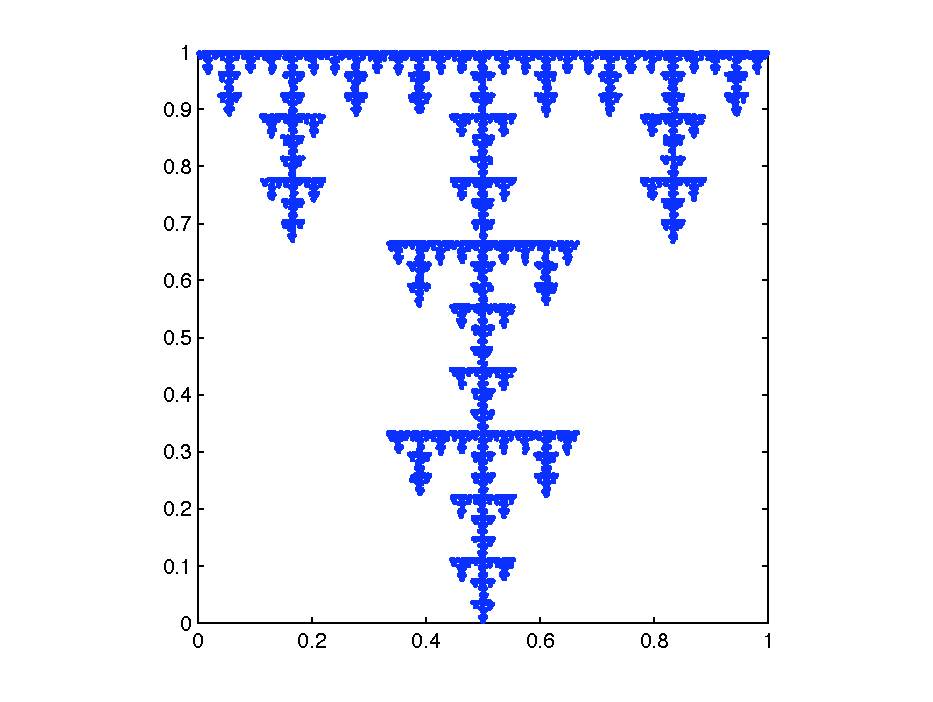
\includegraphics[scale=.5]{Attractor1.pdf}} \atop (I)$ 
\hskip -.6in $\hbox{ 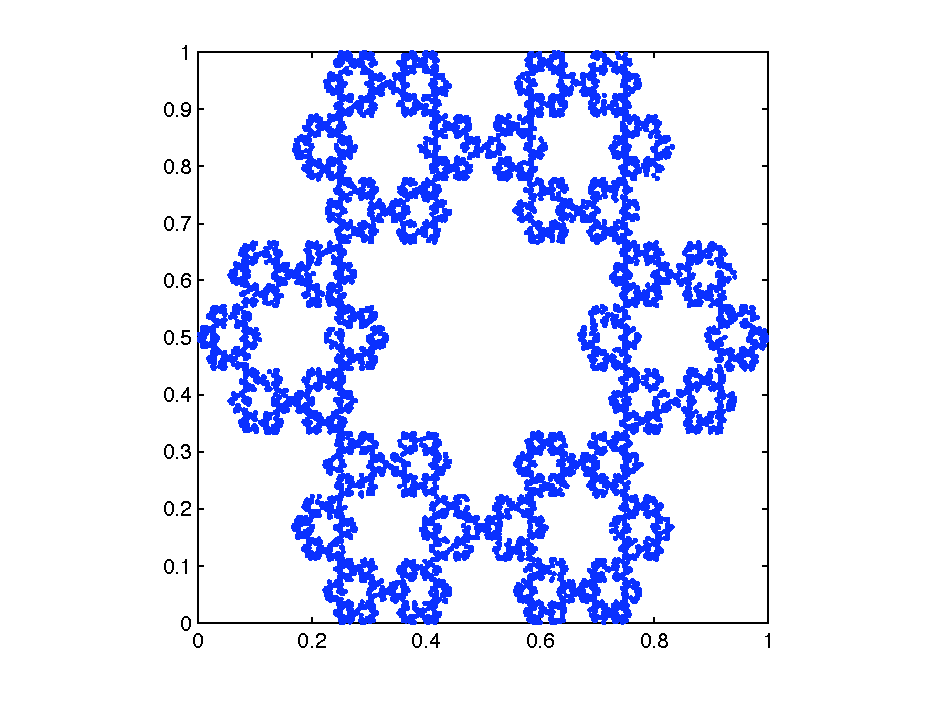
\includegraphics[scale=.5]{Attractor2.pdf}} \atop (II) $ 
\hskip -.6in$\hbox{ 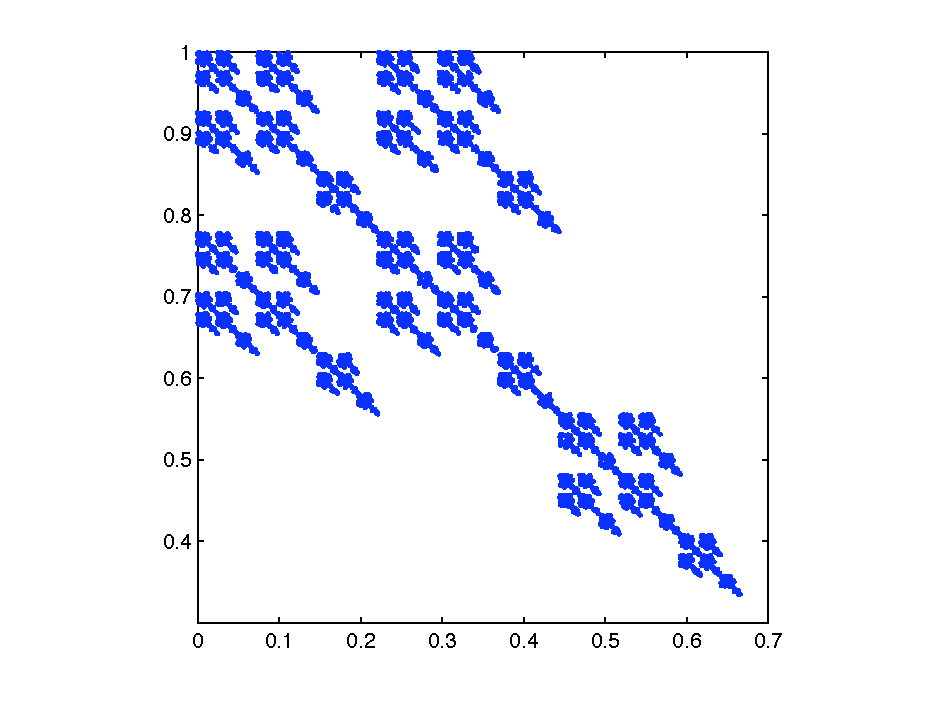
\includegraphics[scale=.5]{Attractor3.pdf}} \atop (III)$}
\vbox{
\hskip -.5in$\hbox{ 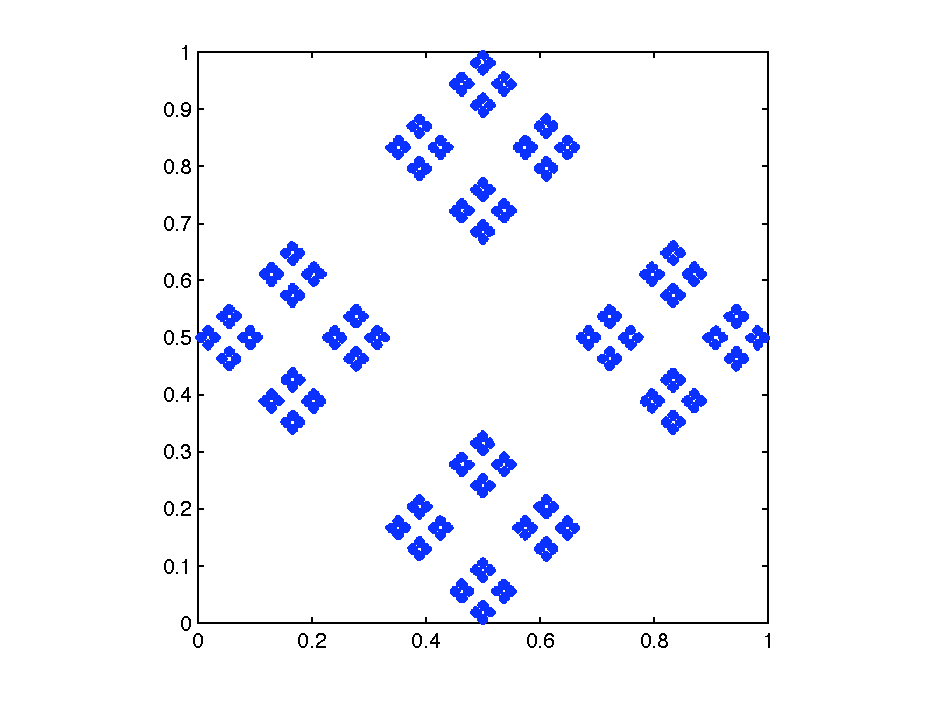
\includegraphics[scale=.5]{Attractor4.pdf}} \atop (IV) $ 
\hskip -.1in $\hbox{ 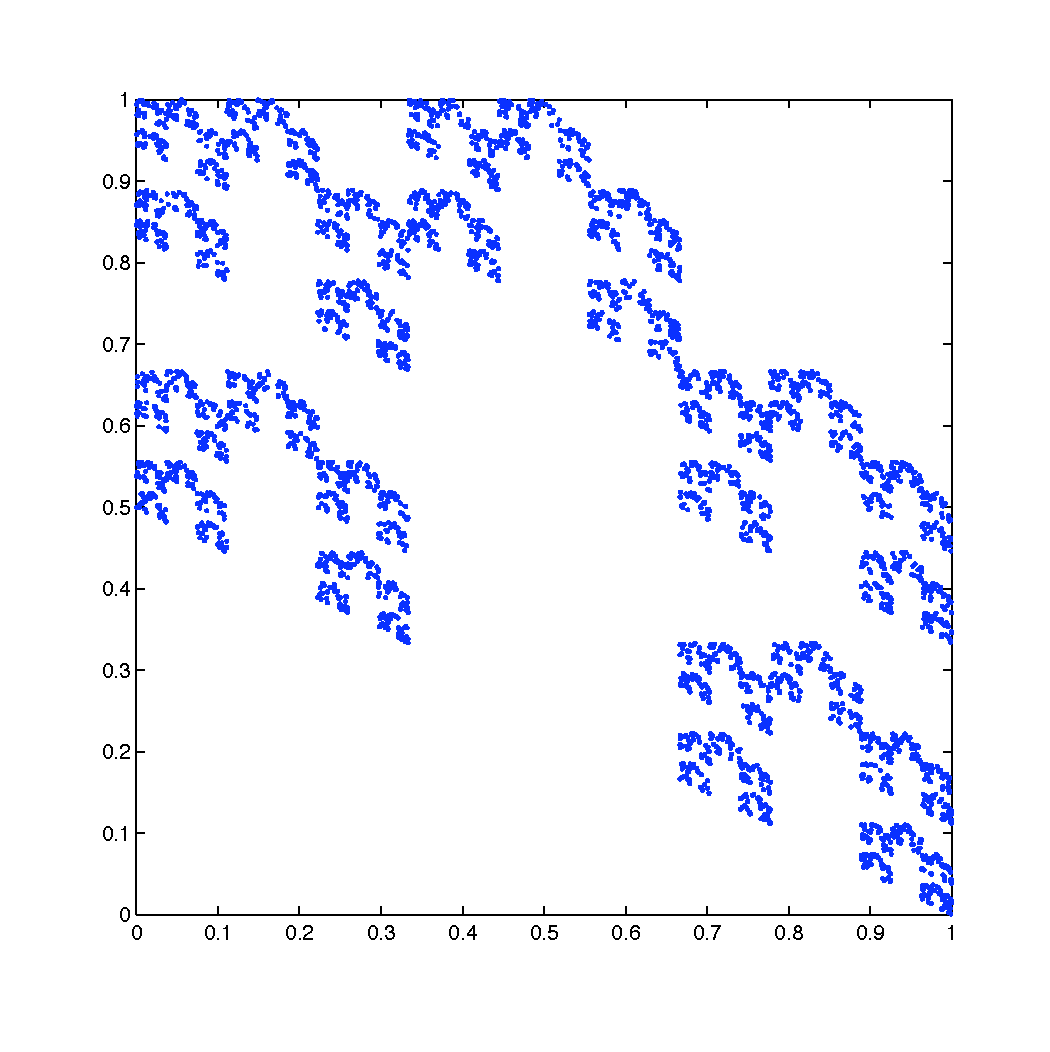
\includegraphics[scale=.35]{Attractor5.pdf}} \atop (V)$ }
\vbox{
\hskip -.2in$\hbox{ 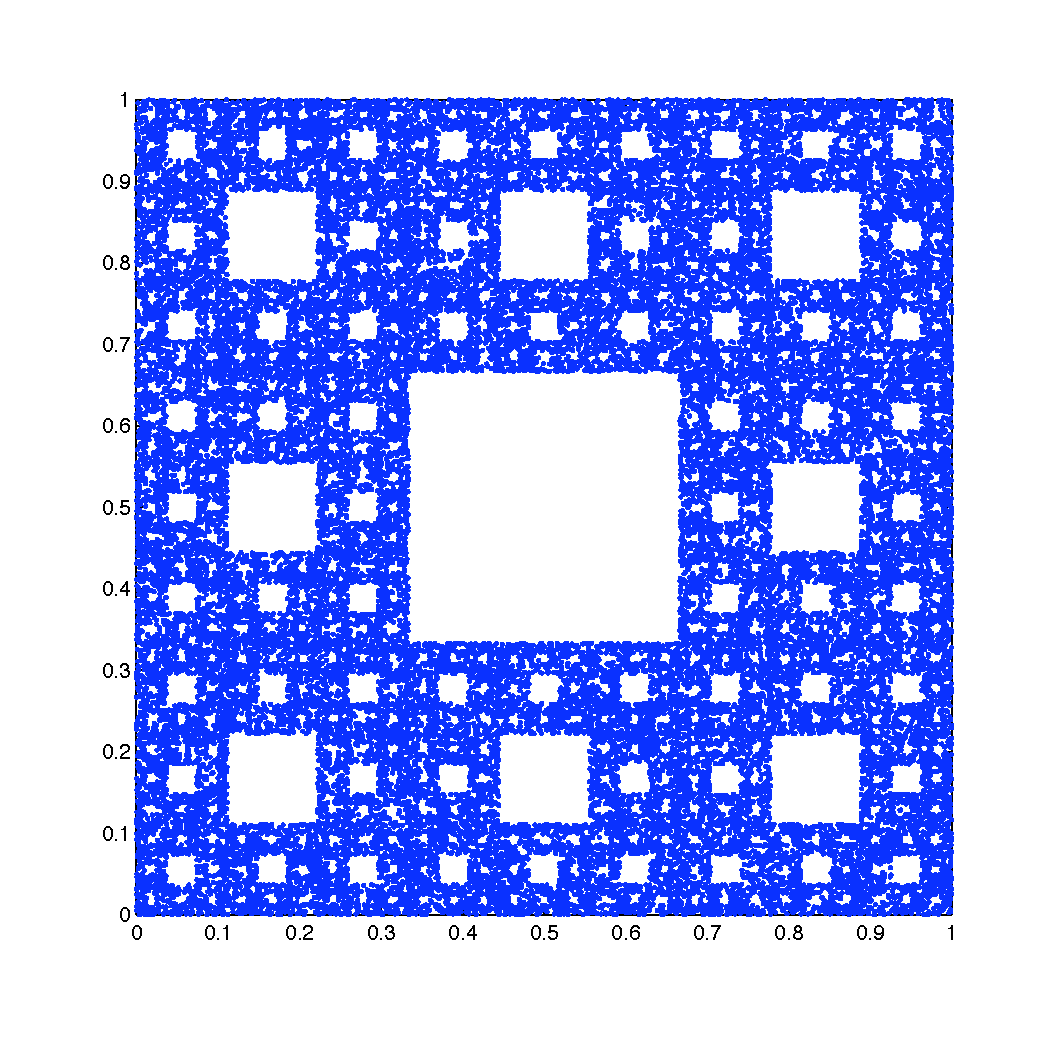
\includegraphics[scale=.35]{Attractor6.pdf}} \atop (VI) $ 
\hskip -.1in $\hbox{ 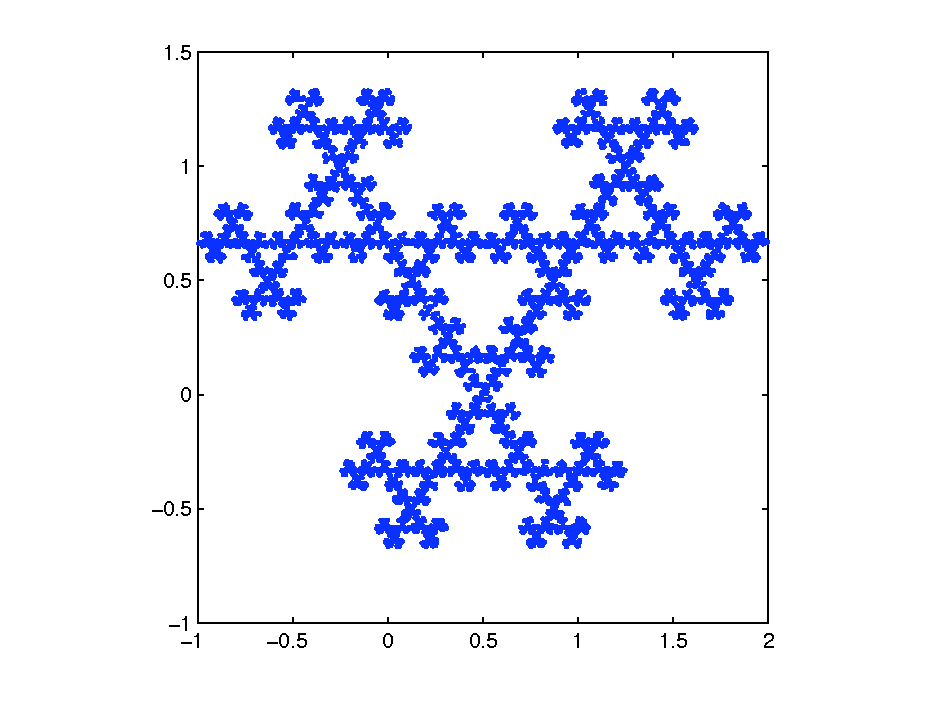
\includegraphics[scale=.5]{Attractor7.pdf}} \atop (VII)$ 
}
\end{enumerate}


\end{document}